\documentclass[12pt]{report}
\usepackage[a4paper]{geometry}
\usepackage[myheadings]{fullpage}
\usepackage{fancyhdr}
\usepackage{lastpage}
\usepackage{graphicx, wrapfig, subcaption, setspace, booktabs}
\usepackage[T1]{fontenc}
\usepackage[font=small, labelfont=bf]{caption}
\usepackage{fourier}
\usepackage[protrusion=true, expansion=true]{microtype}
\usepackage[english]{babel}
\usepackage{sectsty}
\usepackage{url, lipsum}
\usepackage{float}
\usepackage{amsmath}
\usepackage{pdfpages}
\usepackage{amsmath}
\usepackage{amssymb}
\graphicspath{ {./images/}}


\newcommand{\HRule}[1]{\rule{\linewidth}{#1}}
\onehalfspacing
\setcounter{tocdepth}{5}
\setcounter{secnumdepth}{5}

%-------------------------------------------------------------------------------
% HEADER & FOOTER
%-------------------------------------------------------------------------------
\pagestyle{fancy}
\fancyhf{}
\setlength\headheight{15pt}
\fancyhead[L]{Gabriel Colangelo}
\fancyhead[R]{UBID: 50223306}
\fancyfoot[R]{Page \thepage\ of \pageref{LastPage}}
%-------------------------------------------------------------------------------
% TITLE PAGE
%-------------------------------------------------------------------------------

\begin{document}
\title{ \normalsize \textsc{ }
		\\ [2.0cm]
		\HRule{0.5pt} \\
		\LARGE \textbf{Comparison of an Extended and Unscented Kalman Filter for Attitude Estimation Applications}
		\HRule{2pt} \\ [0.5cm]
		\normalsize  \vspace*{5\baselineskip}}



\author{Gabriel Colangelo \\ 
		University at Buffalo \\
		MAE 674} 
\date {12/16/2022}

\maketitle
\tableofcontents
\newpage

%-------------------------------------------------------------------------------
% Section title formatting
\sectionfont{\scshape}
%-------------------------------------------------------------------------------

%-------------------------------------------------------------------------------
% Part 1
%-------------------------------------------------------------------------------
\newpage
\section*{Abstract}
\addcontentsline{toc}{section}{Abstract}
\noindent This paper compares the performance of an Extended Kalman Filters (EKF) and an Unscented Kalman Filter (UKF). The EKFs and UKF were applied to the problem of attitude estimation, or more particularly the dynamic attitude estimation problem. The EKF investigated in this project will be the Multiplicative Extended Kalman Filter, while the UKF investigated in this paper is the Unscented Quaternion Estimator. Both the EKF and UKF were used to estimate the attitude of a rigid body, say a satellite, along with the drift observed in each of the gyroscopes along each axis. The gyroscope measurements were combined with star tracker measurements to create a full dynamic attitude estimation problem. To perform this comparison, all filters were be fed the same initial conditions and sensor measurements. The parameters that were compared are the attitude and gyroscope bias/drift errors and the filter run time. A short study was also done to see each filter’s sensitivity to initial conditions, which was be performed using Monte Carlo simulations.

\newpage
\section*{Introduction}
\addcontentsline{toc}{section}{Introduction}
\noindent The motivation for this proposed project comes from wanting to gain experience in dynamic attitude estimation methods, rather than typical deterministic attitude estimation methods such as the Triad method or Davenport's q-method.  Dynamic attitude estimation involves the combination of attitude measurements at varying times with gyroscope measurements [1]. There are many ways to parameterize attitude such as Euler angles, quaternions, and Rodrigues parameters. For each type of parameterization, specific solutions exist. For example, if attitude is parameterized using Modified Rodrigues Parameters (MRPs), a typical solution is to use an MRP-EKF, which is presented in Schaub and Junkins. Euler Angles are one of the more common choices for attitude parameterization. However, the use of Euler angles comes with a major disadvantage. This disadvantage being that singularities occur in the kinematic differential equations used to calculate Euler Angle rates, when the second rotation angle is equal to $\pm{90^\circ} $ [2]. To avoid this singularity, known as gimbal lock, this paper chooses to use quaternions as the preferred method of attitude parameterization. The kinematic differential equations are linear in the case of quaternions [3], therefore removing the previously discussed singularity and eliminating the need to integrate time consuming trigonometric functions [2].\\

\noindent There are multiple conventions used for quaternion multiplication. This paper chooses to use the convention established by Lefferts, Markley, and Shuster rather than the convention used by Hamilton, who the discovery of the quaternion is typically attributed to [2]. The main difference between these conventions is that the convention used by Lefferts, Markley, and Shuster multiplies quaternions in the same order as the attitude matrices [3]. With the choice of the quaternion as the method for attitude parameterization, the dynamic attitude estimation problem can now be solved by using quaternion based Kalman filter solutions such as the Multiplicative Extended Kalman Filter (MEKF) and the Additive Extended Kalman Filter (AEKF) [1]. A formulation for the MEKF is given in Crassidis and Junkins, and this proposed project will explore its performance and implementation. The MEKF is typically preferred over the AEKF. This is primarily due to the MEKF being less computationally expensive because of the lower dimensionality of its covariance matrix and its attitude estimate being the unit quaternion [4]. Because the AEKF does not naturally satisfy the quaternion unit norm constraint, and the additive correction approach can destroy normalization [5], it will not be used in this paper. Work done by Markley in ref [4] further discuss the issues involved with AEKF.

\noindent The EKF is not considered an optimal estimator and only performs well when a first order linearization can closely approximate nonlinear probability distributions [5]. This approximation tends to break down during initialization when inaccurate initial conditions are used. In this case, it is common to use an Unscented Kalman Filter (UKF). The UKF is more computationally involved than its EKF counterpart, but it provides a variety of benefits. This includes a lower expected error than the EKF, avoiding the computation of the Jacobian, and the UKF is also valid to higher order expansions in comparison to the EKF [5]. A quaternion based UKF is derived in the paper by Crassidis and Markley, which is referred to as the Unscented Quaternion Estimator (USQUE). The UKF may handle large initial condition errors easily, however it does have a downside. A straightforward implementation of the UKF, like the AEKF, does not guarantee the estimated quaternion will satisfy the unit norm constraint and this form of the UKF also involves the decomposition of a 7x7 covariance matrix [6]. The USQUE filter looks to overcome these deficiencies of the normal UKF. This project compares the USQUE performance to that of the MEKF to see if there is one method of quaternion based Kalman filtering that is superior for dynamic attitude estimation.\\

\noindent This paper is broke into four main sections. The first will discuss the measurement and truth models. The second will go through the MEKF algorithm, while the third will go through the USQUE. Lastly, will be the results and discussion where the simulations are shown and investigated. 

\section*{Truth and Measurement Models}
\addcontentsline{toc}{section}{Truth and Measurement Models}
\noindent Both filters were parameterized using the quaternion. The equations governing the quaternion kinematics is shown below [5], where $\pmb{q_I^B}$ is the true quaternion vector and $\pmb{\omega_{B/I}^B}$ is the true angular velocity vector of the body with respect to the inertial frame, expressed in body coordinates.

\begin{equation}
	\Omega(\pmb{\omega_{B/I}^B}) = \begin{bmatrix}
		-[\pmb{\omega_{B/I}^B} \times] & \pmb{\omega_{B/I}^B} \\
		-\pmb{\omega_{B/I}^B}^T & 0
	\end{bmatrix}
\end{equation}  

\begin{equation}
	\pmb{\dot{q}_I^B} = \frac{1}{2}\Omega(\pmb{\omega_{B/I}^B})\pmb{q_I^B}
\end{equation}  

\noindent To generate the true quaternion trajectory, equation 2 was integrated using a 4th order Runge-Kutta integrator and the true angular velocity. \\

\noindent The output of a gyroscope, strap-down gyroscope specifically, is the measured body angular rate relative to the inertial frame expressed in body frame coordinates, denoted by $\pmb{\tilde{\omega}_{B/I}^B}$. A first order Markov process is used for the gyroscope measurement model. This model is given in ref [3] and is also shown below, where $K_g$ is a diagonal matrix of scale factors, $\beta_g$ is the gyroscope bias/drift, $\eta_v$ and $\eta_u$ are zero-mean Gaussian white-noise processes with their respective spectral densities $\sigma_v^2 I_{3\times3}$ and $\sigma_u^2 I_{3\times3}$.

\begin{equation}
\pmb{\tilde{\omega}_{B/I}^B} = (I_{3\times3} + K_g)\pmb{\omega_{B/I}^B} + \pmb{\beta_g} + \pmb{\eta_v}
\end{equation}

\begin{equation}
	\pmb{\dot{\beta}_g} = \pmb{\eta_u}
\end{equation}

\noindent This model is a continuous time model, which is difficult for computer simulation. Therefore, a discrete time single axis gyroscope measurement model to be used for simulation is shown below, where the scale factors are assumed to be zero [3]. 

\begin{equation}
\tilde{\omega}_{k+1} = \omega_{k+1} + \frac{1}{2}[\beta_{k+1} + \beta_k] + [\frac{\sigma_v^2}{\Delta t} + \frac{1}{12}\sigma_u^2 \Delta t]^\frac{1}{2} N_V
\end{equation}

\begin{equation}
	\beta_{k+1} = \beta_k + \sigma_u \Delta t^\frac{1}{2} N_u
\end{equation}

\noindent Equations 5 and 6 show that the gyroscope measurements and bias can be discretely propagated using the true angular velocity. In these equations, it should be noted that $N_v$ and $N_u$ are both zero-mean random variables with unit variance [3]. The other sensor used in the simulation is a star tracker. A star tracker measurement model is given in ref [5]. Each body frame star measurement, $\tilde{b}_j$, can be given by

\begin{equation}
	\tilde{b}_j = A_I^B\pmb{r}_j + v_j     
\end{equation}

\noindent In this expression, j goes from 1 to the number of star observations, $v_j$ is the approximately Gaussian sensor error, $A_I^B$ is the true quaternion parameterized attitude matrix, and $r_j$ is the inertial/reference frame vector. The sensor error is assumed to be zero mean with variance $\sigma_n^2$. The reference frame vectors can be determined from the spherical coordinate angles $\alpha$ and $\delta$, which are the right ascension and declination angles respectively. The stars being tracked are assumed to be inertially fixed [5]. The equations used to determine the reference vectors from the spherical ascension and declination angles are given below.
\begin{equation}
	r_{xj} = \cos(\delta_j) \cos(\alpha_j)   
\end{equation}
\begin{equation}
	r_{yj} = \cos(\delta_j) \sin(\alpha_j)   
\end{equation}
\begin{equation}
	r_{zj} = \sin(\delta_j)  
\end{equation}
\begin{equation}
	\pmb{r}_j = [r_{xj},r_{yj},	r_{zj}] ^T
\end{equation}

\noindent The last component needed to find each star measurement is the attitude matrix. The true propagated quaternion can be used to compose an attitude matrix using the equations below where $\pmb{\rho}$ is the vector part of the quaternion and $q_4$ is the scalar part [6]. 

\begin{equation}
	\pmb{q}_I^B = [\pmb{\rho}, q_4]^T
\end{equation}

\begin{equation}
	\Xi(\pmb{q}_I^B)= \begin{bmatrix}
		q_4I_{3\times3} + [\pmb{\rho}\times] \\
		-\pmb{\rho}^T
	\end{bmatrix}
\end{equation}

\begin{equation}
	\Psi(\pmb{q}_I^B)= \begin{bmatrix}
		q_4I_{3\times3} - [\pmb{\rho}\times] \\
		-\pmb{\rho}^T
	\end{bmatrix}
\end{equation}

\begin{equation}
	A_I^B(\pmb{q}_I^B) = \Xi^T\Psi
\end{equation}

\noindent This section has reviewed the equations and models used to propagate star tracker and gyroscope measurements. These measurements will now be used in the MEKF and USQUE filters, starting with the MEKF in the next section.

\section*{Multiplicative Extended Kalman Filter}
\addcontentsline{toc}{section}{Multiplicative Extended Kalman Filter}

\noindent As previously discussed, when using quaternions to parameterize the attitude, the quaternion unit norm constraint must be satisfied. Therefore, when using an Extended Kalman Filter for attitude estimation it is better to use a multiplicative error quaternion in the body frame to preserve normalization, as the additive error quaternion can destroy normalization [5]. This is the basis of the MEKF. The algorithm for the MEKF is as follows [5]. First, the estimates for the quaternion ($\pmb{\hat{q}}_0$) and the gyroscope bias ($\hat{\beta}_0$) are initialized, along with the state error covariance matrix ($P_0$). The initial state error covariance is a diagonal 6x6 matrix (to be discussed shortly) consisting of the initial attitude ($P_0^a$) and gyro drift/bias covariance ($P_0^b$), as shown below.

\begin{equation}
	P_0 = \begin{bmatrix}
		P_0^a & 0 & 0 & 0 & 0 & 0 \\
		0 & P_0^a & 0 & 0 & 0 & 0 \\
		0 & 0 & P_0^a & 0 & 0 & 0\\
		0 & 0 & 0 & P_0^b & 0 & 0 \\
		0 & 0 & 0 & 0 & P_0^b & 0 \\
		0 & 0 & 0 & 0 & 0 & P_0^b	
	\end{bmatrix}
\end{equation}

\noindent The measurement noise covariance (R) and the discrete process noise covariance ($Q_k$) are given below, where $\sigma_{n}$ is the star tracker noise parameter for the $n^{th}$ vector/star measurement,  and $\sigma_v$  and $\sigma_u$ are the gyroscope noise parameters. 

\begin{equation}
	R = diag[\sigma_1^2I_{3\times3} ... \sigma_n^2I_{3\times3}]
\end{equation}


\begin{equation}
	Q_k = \begin{bmatrix}
	(\sigma_v^2 \Delta t + \frac{1}{3}\sigma_u^2\Delta t^3)I_{3\times3} & (\frac{1}{2}\sigma_u^2\Delta t^2)I_{3\times3}\\
	(\frac{1}{2}\sigma_u^2\Delta t^2)I_{3\times3} & (\sigma_u^2\Delta t)I_{3\times3}
	
	\end{bmatrix}
\end{equation}


\noindent It should be noted that the measurement noise covariance matrix is clearly an nxn diagonal block matrix, and that the discrete process noise covariance was chosen over the process noise spectral density matrix, Q(t). This was done so that the state error covariance could be discretely propagated. With the covariance matrices defined, the Kalman gain can be determined. First, the sensitivity matrix, $H_k$, is calculated with the following relation where $A(\pmb{\hat{q}^{-1}})$ is the attitude matrix generated from equations 12 -15 using the predicted quaternion estimate, $\pmb{\hat{q}^{-1}}$, and $\pmb{r_n}$ is the reference frame unit vector for each star measurement . Please note that the subscripts and superscripts of I and B respectively, have been dropped from the notation of the quaternion and attitude matrix for the sake of length. 

\begin{equation}
	H_k = \left. \begin{bmatrix}
		[A(\pmb{\hat{q}^{-1}})\pmb{r_1}\times] & 0_{3\times3}\\
		. & . \\
		. & . \\
		. & . \\
		[A(\pmb{\hat{q}^{-1}})\pmb{r_n}\times] & 0_{3\times3}]
			
	\end{bmatrix}\right|_{t_k} =  \left. \frac{\partial\pmb{h}}{\partial\pmb{x}}\right|_{\hat{\pmb{x}}_k^-}
\end{equation}

\noindent The equation for the Kalman gain is given below, where $P_k^-$ is the predicted error covariance, and is initially equal to $P_0$ for the first time step.

\begin{equation}
	K_k = P_k^- H_k^T[H_KP_k^-H_k^T + R]^{-1}
\end{equation}

\noindent It should be noted that the sensitivity matrix has 6 columns. This is due to the same reason the error covariance matrix is a 6x6 matrix. The reason is that a reduced order state error model is being used in place of the full exact kinematic relationship for the attitude errors, given by equation 7.13 in ref [5]. To get the reduced state error model two approximations are made. The first approximation is that the fourth error quaternion component is constant in the first order linearization of equation 7.13 of ref [5]. This linearized model maintains the quaternion norm within the first order approximation in the EKF. The second is that the small angle approximation is made such that the vector component of the error quaternion ($\delta\pmb{\rho}$) is approximately equal to a vector of error half angles($\delta\pmb{\alpha}/2$) where $\delta\pmb{\alpha}$ has components of yaw, pitch, and roll errors. The attitude error component of the error model has now been reduced from ($\delta\pmb{q}$) = $ [(\delta\pmb{\rho}) \delta q_4] ^T$ (4 states) to $\delta\pmb{\alpha}$ (3 states) as $\delta q_4$ is approximately 1. Ultimately, the full vector of state errors is given by $\Delta\pmb{\hat{\tilde{x}}_k^+} = [\delta\pmb{\hat{\alpha}}_k^{+T} \Delta\hat{\beta}_k^{+T}]^T$, where $\Delta\beta$ is the 3x1 bias error vector. The linearized MEKF error model is now given by:

\begin{equation*}
	\delta\dot{\pmb{\alpha}} =-[\hat{\pmb{\omega}}\times]\delta{\pmb{\alpha}} - \Delta\beta+\eta_v
\end{equation*}


\noindent With the Kalman gain calculated and the state errors defined, the update stage of the MEKF can be performed. The error covariance is updated with the equation

\begin{equation}
	P_k^+ =[I - K_kH_k]P_k^-
\end{equation}

\noindent The estimated output $h_k$ is given by the following expression

\begin{equation}
	\pmb{h_k} = \left. \begin{bmatrix}
		A(\pmb{\hat{q}^{-1}})\pmb{r_1} \\
		.  \\
		. \\
		. \\
		A(\pmb{\hat{q}^{-1}})\pmb{r_n}
		
	\end{bmatrix}\right|_{t_k}
\end{equation}

\noindent With the estimated output, the state errors can be updated with the star measurements, $\tilde{b}$ from equation 7 and the Kalman gain. The equation used to calculate the estimated state update error is

\begin{equation}
	\Delta\pmb{\hat{\tilde{x}}}_k^+ = K_k[\tilde{\pmb{b}}_k - \pmb{h_k}]
\end{equation}

\noindent With the estimated error state update found, the quaternion and bias can now be updated. The equations for the updated quaternion and bias are given below. It should be noted that the updated quaternion is normalized after the update if the norm diverges by greater than $10^{-7}$ from unit norm.

\begin{equation}
	\pmb{\hat{q}}_k^+ = \pmb{\hat{q}}_k^- + \frac{1}{2}\Xi(\hat{\pmb{q}}_k^-)\delta\hat{\pmb{\alpha}}_k^+
\end{equation}

\begin{equation}
	\hat{\beta}_k^+ = \hat{\beta}_k^- + \Delta\hat{\beta}_k^{+T}
\end{equation}

\noindent With the update stage complete, the predicted quaternion, bias, and error covariance for the next time step can now be propagated. First, the post updated angular velocity is calculated with the expression below, where $\tilde{\pmb{\omega}}_k$ is the vector of gyroscope measurements from equation 5. 

\begin{equation}
	\hat{\pmb{\omega}}_k^+ = \tilde{\pmb{\omega}}_k - \hat{\beta}_k^+
\end{equation}

\noindent The bias propagation is given by

\begin{equation}
	\hat{\beta}_{k+1}^- = \hat{\beta}_k^+
\end{equation}

\noindent as 

\begin{equation}
	\dot{\hat{\beta}} = \pmb{0}  
\end{equation}

\noindent Using the updated angular velocity, the propagated quaternion, $\hat{q}_{k+1}^-$, can be found by numerically integrating the quaternion kinematics below using a Runge-Kutta integrator at each time step. 

\begin{equation}
	\pmb{\dot{\hat{q}}} = \frac{1}{2}\Omega(\hat{\pmb{\omega}}_k^+)\pmb{\hat{q}}_k^+
\end{equation}  

\noindent As mentioned prior, the error covariance will be discretely propagated. To do this the error model matrices F and G must be converted to their discrete time equivalents $\Phi_k$ and $\Upsilon_k$. $\Upsilon_k$ is simply 

\begin{equation}
	\Upsilon_k= \begin{bmatrix}
	-I_{3\times3} & 0_{3\times3} \\
	0_{3\times3} & I_{3\times3}
	\end{bmatrix}
\end{equation}

\noindent The transformation of F to its discrete error state transition matrix $\Phi_k$ requires taking the matrix exponential of the product of F and the sampling period $\Delta t$. F is found from the MEKF error model and is given by,

\begin{equation}
	F = \begin{bmatrix}
		-[\hat{\pmb{\omega}}_k^+\times] & -I_{3\times3}\\
		0_{3\times3} & 0_{3\times3}
	\end{bmatrix}
\end{equation}

\noindent Therefore, $\Phi_k$ is given by 
\begin{equation}
	 \Phi_k = e^{F\Delta t}
\end{equation}  

\noindent Now with $\Phi_k$ and $\Upsilon_k$ determined, the propagated error covariance can be calculated with the equation below.  

\begin{equation}
	P_{k+1}^- = \Phi_kP_k^+\Phi_k^T + \Upsilon_kQ_k\Upsilon_k^T
\end{equation}  

\noindent This completes the MEKF algorithm [5]. This algorithm takes in the initial conditions then  runs through each time step accordingly to propagate the states and error covariance using a multiplicative error quaternion.  It should be noted that taking the square root of the diagonal of $P^-$ and multiplying by 3 gives the 3$\sigma$ error bounds. The last thing to mention before moving onto the USQUE algorithm, is how the attitude errors are calculated. The error quaternion is given by

\begin{equation}
	\delta\pmb{q} = \pmb{q} \otimes \hat{\pmb{q}}^{-1}
\end{equation}  

\noindent where $\pmb{q}$ is the true quaternion and $\pmb{\hat{q}}^{-1}$ is the inverse of the estimated quaternion from equation 24. The inverse of the quaternion is 

\begin{equation}
\pmb{q}^{-1} = \begin{bmatrix}
	-\pmb{\rho} \\
	 q_4
	 \end{bmatrix}
\end{equation}  

\noindent The quaternion multiplication is bi-linear and is performed by

\begin{equation}
 \pmb{q} \otimes \hat{\pmb{q}}^{-1} = \begin{bmatrix}
 	\Xi(\hat{\pmb{q}}^{-1}) & \hat{\pmb{q}}^{-1}
 \end{bmatrix}\pmb{q}
\end{equation}  

\section*{Unscented Quaternion Estimator}
\addcontentsline{toc}{section}{Unscented Quaternion Estimator}
\noindent The USQUE is a based on the Unscented Kalman Filter, which uses sample points to map the probability distribution [6]. This differs from the Extended Kalman Filter which relies on the linearization giving a good approximation of the non-linear probability distribution. A standard UKF using the quaternion kinematics shown in equation 2, doesn't guarantee to produce a quaternion estimate that satisfies the unit norm constraint unless done by brute force [6]. It also produces a 7x7 error covariance matrix which is more computationally expensive to decompose than the 6x6 covariance matrix introduced in the MEKF section of this paper. To reduce the size of the covariance matrix and guarantee unit norm, the USQUE was derived in ref [6]. In the USQUE, the global attitude is still parameterized by the quaternion and the multiplicative error quaternion is used to guarantee that the quaternion unit norm constraint is satisfied. However, an unconstrained three-dimensional vector of Rodrigues parameters is used to define the attitude error quaternion. This three component representation of the quaternion guarantees the quaternion estimate has unit norm and produces a 6x6 covariance matrix [6]. Classical Rodrigues parameters/Gibbs vector are a minimal three parameter set that have a singularities that occur at $\pm 180^\circ$. A projection from the quaternion unit norm constrained sphere to the three-dimensional hyperplane is given in ref [1]. This projection yields the transformation from quaternions to classical Rodrigues parameters. This transformation is given below.

\begin{equation}
	\pmb{p} = \frac{\pmb{\rho}}{q_4}
\end{equation}  

\noindent The transformation from quaternions to the generalized Rodrigues parameters is shown below where f is a scale factor and a ranges from 0 to 1.  

\begin{equation}
	\pmb{p} = f \frac{\pmb{\rho}}{a + q_4}
\end{equation} 

\noindent or in terms of the error quaternion

 \begin{equation}
 	\pmb{\delta p} = f \frac{\pmb{\delta\rho}}{a + \delta q_4}
 \end{equation} 

\noindent If f = 1 and a = 0, we see that equation 38 yields equation 37, i.e. the transformation from the quaternios to the Gibbs vector. Equation 39 will be used to relate the error quaternion to the local attitude error represented by the generalized Rodrigues parameters. For the USQUE, f is be chosen to be f = (2a + 1) [6]. Now with the covariance matrix reduced to a 6x6 and the quaternion norm constraint discussed, the algorithm of the USQUE will be presented. First, using the initial error covariance matrix from equation 16 and setting $P_0 = P_k^+$, the matrix square root is performed using a Cholesky decomposition. It should be noted that there are 2n sigma points (n is the dimension of $P_k^+$) due to the positive and negative components of the square root. 

 \begin{equation}
	\sigma_k = \pm\sqrt{(n+\lambda)[P_k^+ + \bar{Q}_k]}
\end{equation} 

\noindent $\lambda$ is the filter tuning parameter and $\bar{Q}_k$ is given by


\begin{equation}
	\bar{Q}_k = \frac{\Delta t}{2}\begin{bmatrix}
		(\sigma_v^2 - \frac{1}{6}\sigma_u^2\Delta t^2)I_{3\times3} & 0_{3\times3} \\
		0_{3\times3} & \sigma_u^2I_{3\times3}
	\end{bmatrix}
\end{equation} 

\noindent Using the state vector, the sigma points are found with the relation below. It should be noted that for the first iteration, the initial state vector is $\pmb{\hat{x}}_0^+$ = $[\pmb{0}^T,  \hat{\beta}_0^T]^T$ where $\hat{\beta}_0$ is the initial gyro bias/drift estimate, and the initial quaternion estimate is given by $\pmb{\hat{q}}_0$ (same initial estimates as in the MEKF section). 

 \begin{equation}
	\pmb{\chi}_k(0) = \pmb{\hat{x}}_k^+ = \begin{bmatrix} \delta\hat{\pmb{p}}_k^+ \\ \hat{\beta}_k^+
		\end{bmatrix}
\end{equation} 


 \begin{equation}
	\pmb{\chi}_k(i) = \sigma_k(i) +  \pmb{\hat{x}}_k^+
\end{equation} 

\noindent All 2n+1 sigma points are partitioned into a vector, as shown below.

\begin{equation}
	\pmb{\chi}_k(i) = \begin{bmatrix} \pmb{\chi}_k^{\delta p}(i) \\ \pmb{\chi}_k^{\beta}(i)
	\end{bmatrix} \quad 	i = 0,1,..12
\end{equation} 

\noindent Next, the sigma point quaternions and error quaternions are calculated with the following relations.

 \begin{equation}
	\delta q_{4k}^+(i) = \frac{-a||\pmb{\chi}_k^{\delta p}(i)||^2 + f \sqrt{f^2 + (1 - a^2)||\pmb{\chi}_k^{\delta p}(i)||^2}}{f^2 + ||\pmb{\chi}_k^{\delta p}(i)||^2} \quad i = 1,2,..12
\end{equation} 

 \begin{equation}
	\delta \pmb{\rho}_k^+(i) = f^{-1} [a + \delta q_{4k}^+(i)]\pmb{\chi}_k^{\delta p}(i) \quad i = 1,2,..12
\end{equation} 

\begin{equation}
\delta\pmb{q}_k^+(i)  = \begin{bmatrix} 	\delta \pmb{\rho}_k^+(i) \\ 	\delta q_{4k}^+(i)
\end{bmatrix}
\end{equation} 

\begin{equation}
\pmb{q}_k^+(0)  = \pmb{q}_k^+
\end{equation} 

\begin{equation}
	\pmb{q}_k^+(i)  = \delta\pmb{q}_k^+(i) \otimes \pmb{q}_k^+ \quad i = 1,2,..12
\end{equation} 

\noindent Next, the estimated angular velocity is found using the gyroscope output and the equation below.

\begin{equation}
	\pmb{\hat{\omega}}_k^+(i)  = \tilde{\pmb{\omega}}_k - \pmb{\chi}_k^{\beta}(i) \quad i = 0,1,..12
\end{equation} 

\noindent With the estimated angular velocities found, each sigma point quaternion can be propagated in time to obtain $\hat{\pmb{q}}_{k+1}^-(i)$ by numerically integrating the quaternion kinematics from the equation below, where $\pmb{q}_k^+(i)$ is a 4x13 concatenated matrix with entries made from the outputs of equations 48 and 49.

\begin{equation}
	\pmb{\dot{\hat{q}}} = \frac{1}{2}\Omega[\pmb{\hat{\omega}}_k^+(i)]\pmb{q}_k^+(i) \quad i = 0,1,..12
\end{equation} 

\noindent After using a 4th order Runge-Kutta integrator to find $\hat{\pmb{q}}_{k+1}^-(i)$ from the output of equation 51, the propagated error quaternion can computed with the equation 

\begin{equation}
	\delta\pmb{q}_{k+1}^-(i) = \pmb{q}_{k+1}^-(i) \otimes [\pmb{q}_{k+1}^-(0)]^{-1} \quad i = 0,1,..12
\end{equation} 

\noindent Now the propagated sigma points can be found using the relations

\begin{equation}
	 \pmb{\chi}_{k+1}^{\delta p}(0) = \pmb{0}
\end{equation}

\begin{equation}
	\delta\pmb{q}_{k+1}^-(i)  = \begin{bmatrix} 	\delta \pmb{\rho}_{k+1}^-(i) \\ 	\delta q_{4,k+1}^-(i)
	\end{bmatrix}
\end{equation} 

\begin{equation}
	\pmb{\chi}_{k+1}^{\delta p}(i) = f \frac{\delta\pmb{\rho_{k+1}^-(i)}}{a + \delta q_{4,k+1}^-(i)} \quad i = 1,2,..12
\end{equation}

\begin{equation}
	\pmb{\chi}_{k+1}^{\beta}(i) = \pmb{\chi}_{k}^{\beta}(i) \quad i = 0,1,..12
\end{equation}

\noindent With the propagated sigma points determined, the predicted mean and covariance are found with the equations below. 

\begin{equation}
	\hat{\pmb{x}}_{k+1}^- = \frac{1}{n + \lambda} [\lambda\pmb{\chi}_{k+1}(0) + \frac{1}{2}\sum_{i =1}^{2n}\pmb{\chi}_{k+1}(i)]
\end{equation}

\begin{equation}
	{\pmb{P}}_{k+1}^- = \frac{1}{n + \lambda} [\lambda (\pmb{\chi}_{k+1}(0) - \hat{\pmb{x}}_{k+1}^-)
	(\pmb{\chi}_{k+1}(0) - \hat{\pmb{x}}_{k+1}^-)^T + \frac{1}{2}\sum_{i =1}^{2n}(\pmb{\chi}_{k+1}(i) - \hat{\pmb{x}}_{k+1}^-)
	(\pmb{\chi}_{k+1}(i) - \hat{\pmb{x}}_{k+1}^-)^T] + \bar{Q}_k
\end{equation}

\noindent Using the propagated quaternions, $\hat{\pmb{q}}_{k+1}^-(i)$, from equation 51 the estimated output for each propagated quaternion is given by

\begin{equation}
	\pmb{\gamma}_{k+1}(i) = \left. \begin{bmatrix}
		A(\hat{\pmb{q}}_{k+1}^-(i))\pmb{r_1}\\
		.  \\
		. \\
		. \\
		A\hat{\pmb{q}}_{k+1}^-(i))\pmb{r_n}
		
	\end{bmatrix}\right|_{k+1} = \pmb{h}[\pmb{\chi}_{k+1}(i)] \quad i = 0,1,..12
\end{equation}

\noindent With the estimated output, the mean observation can be calculated with 

\begin{equation}
	\hat{\pmb{y}}_{k+1}^- = \frac{1}{n + \lambda} [\lambda\pmb{\gamma}_{k+1}(0) + \frac{1}{2}\sum_{i =1}^{2n}\pmb{\gamma}_{k+1}(i)]
\end{equation}

\noindent Next the output covariance, innovation covariance, and cross-correlation matrix are found using the following, where R is given by equation 17.

\begin{equation}
	{\pmb{P}}_{k+1}^{yy} = \frac{1}{n + \lambda} [\lambda (\pmb{\gamma}_{k+1}(0) - \hat{\pmb{y}}_{k+1}^-)
	(\pmb{\gamma}_{k+1}(0) - \hat{\pmb{y}}_{k+1}^-)^T + \frac{1}{2}\sum_{i =1}^{2n}(\pmb{\gamma}_{k+1}(i) - \hat{\pmb{y}}_{k+1}^-)
	(\pmb{\gamma}_{k+1}(i) - \hat{\pmb{y}}_{k+1}^-)^T] 
\end{equation}

\begin{equation}
	{\pmb{P}}_{k+1}^{vv} = {\pmb{P}}_{k+1}^{yy} + R_{k+1}
\end{equation}

\begin{equation}
	{\pmb{P}}_{k+1}^{xy} = \frac{1}{n + \lambda} [\lambda (\pmb{\chi}_{k+1}(0) - \hat{\pmb{x}}_{k+1}^-)
	(\pmb{\gamma}_{k+1}(0) - \hat{\pmb{y}}_{k+1}^-)^T + \frac{1}{2}\sum_{i =1}^{2n}(\pmb{\chi}_{k+1}(i) - \hat{\pmb{x}}_{k+1}^-)
	(\pmb{\gamma}_{k+1}(i) - \hat{\pmb{y}}_{k+1}^-)^T] 
\end{equation}

\noindent Next, the Kalman gain can be found with the equation below.

\begin{equation}
	K_{k+1} = 	{\pmb{P}}_{k+1}^{xy} ({\pmb{P}}_{k+1}^{vv})^{-1}
\end{equation}

\noindent The innovation is given below, where $\tilde{b}$ is the star tracker output.

\begin{equation}
	\pmb{\nu}_{k+1} = \tilde{\pmb{b}}_{k+1} - \hat{\pmb{y}}_{k+1}^- = \tilde{\pmb{b}}_{k+1} - \pmb{h}(\hat{\pmb{x}}_{k+1}^-)
\end{equation}

\noindent Finally, the state vector and error covariance are updated with the equations 

\begin{equation}
	\hat{\pmb{x}}_{k+1}^+ = \hat{\pmb{x}}_{k+1}^- + K_{k+1} \pmb{\nu}_{k+1}
\end{equation}

\begin{equation}
	P_{k+1}^+ = P_{k+1}^-  - K_{k+1}P_{k+1}^{vv} K_{k+1}^T
\end{equation}

\noindent Now with the state vector updated, the quaternion can appropriately be updated using the following. Again partitioning the state vector in the same fashion as equation 42 the error quaternion is found by

 \begin{equation}
	\delta q_{4,k+1}^+ = \frac{-a||\delta\pmb{p}_{k+1}^+||^2 + f \sqrt{f^2 + (1 - a^2)||\delta\pmb{p}_{k+1}^+||^2}}{f^2 + ||\delta\pmb{p}_{k+1}^+||^2} 
\end{equation} 

\begin{equation}
	\delta \pmb{\rho}_{k+1}^+ = f^{-1} [a + \delta q_{4,k+1}^+]\delta\pmb{p}_{k+1}^+
\end{equation} 

\begin{equation}
	\delta\pmb{q}_{k+1}^+  = \begin{bmatrix} 		\delta \pmb{\rho}_{k+1}^+ \\ 	\delta q_{4,k+1}^+
	\end{bmatrix}
\end{equation} 

\noindent $\delta\pmb{p}_{k+1}^+$ is reset to zero for the next time step, and the quaternion is updated using the equation below. 


\begin{equation}
	\hat{\pmb{q}}_{k+1}^+ = \delta\pmb{q}_{k+1}^+ \otimes \hat{\pmb{q}}_{k+1}^-(0)
\end{equation} 

\noindent This completes the USQUE algorithm. The quaternion update is normalized in a similar to fashion as to what was done in the MEKF if the norm diverges by more than $10^{-7}$. The quaternion error to be used for the computation of the yaw, pitch, and roll attitude errors, can be calculated using equation 36. The next section will discuss the implementation of both the MEKF and USQUE in simulation.

\section*{Single Run Simulation }
\addcontentsline{toc}{section}{Single Run Simulation}
\noindent Both the single run and Monte Carlo runs used the same truth and noise parameters. The true angular velocity is given by

\begin{equation}
	\pmb{\omega_{B/I}^B} = 0 \hat{\pmb{b}}_1 + 90 \hat{\pmb{b}}_2 + 30 \hat{\pmb{b}}_3 \quad [deg/hr]
\end{equation} 

\noindent The true initial quaternion is given by $\pmb{q_0} = [0.0144, .7070, .7070, 0.0144]^T$. The true quaternion and body angular velocity trajectories over an one hour period is given in the figures below. 
\newpage

\begin{figure}[h!]
	\centering
	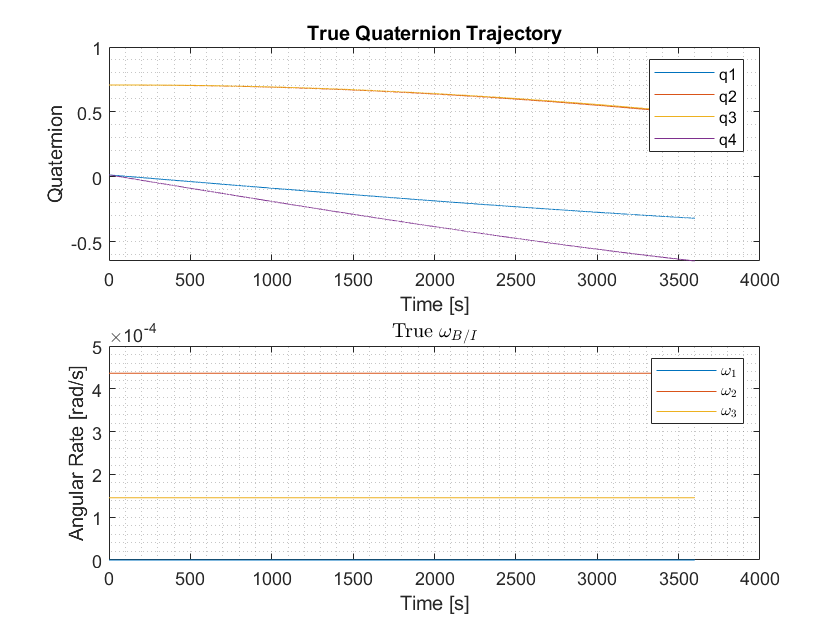
\includegraphics[width = .8\textwidth]{Truth.png}
	\caption{True Quaternion and Angular Velocity Trajectories}
	\label{fig:Part B}
\end{figure}

\noindent As previously mentioned, the attitude estimation problem involves a gyroscope and a star tracker. The gyroscope and star tracker noise parameters are given in the table below. 

\begin{table}[h]
	\begin{center}
		\caption{Noise Parameters }
		\begin{tabular}{|c|c|}
			\hline
			$\sigma_n$ & $3x10^{-5} \quad [rad]$ \\
			\hline
			$\sigma_v$ & $\sqrt{10}x10^{-7} \quad [\frac{rad}{s^{1/2}}]$  \\
			\hline
			$\sigma_u$ & $\sqrt{10}x10^{-10} \quad  [\frac{rad}{s^{3/2}}]$ \\
			\hline

		\end{tabular}
		\label{table:noise parameters}
	\end{center}
\end{table}  

\noindent For the star tracker, a total of 5 stars were sensed continuously. Using the noise parameters from table 1, 5 star vector measurements were made continuously over the one hour period. The spherical coordinates declination and right ascension angles for each star tracked is given in the table below. 
\newpage
\begin{table}[h]
	\begin{center}
		\caption{Star Spherical Coordinate Angles}
		\begin{tabular}{|c|c|c|}
			\hline
			Star \# & Declination [deg] & Right Ascension [deg] \\
			\hline
			1 & 0 & 0  \\
			\hline
			2 & 15 & 30  \\
			\hline
			3 & 30 & 45  \\
			\hline
			4 & 45 & 60  \\
			\hline
			5 & 60 & 75  \\
			\hline
		\end{tabular}
		\label{table: star angles}
	\end{center}
\end{table}  

\noindent Using equations 5,6, and the noise parameters in table 1, the gyroscope measurements and bias for each axis were generated from the true angular velocity trajectory. The initial gyro bias for each axis was set to 0.1 deg/hr. The gyro output and bias is shown below. 

\begin{figure}[h!]
	\centering
	\begin{minipage}{.5\textwidth}
		\centering
		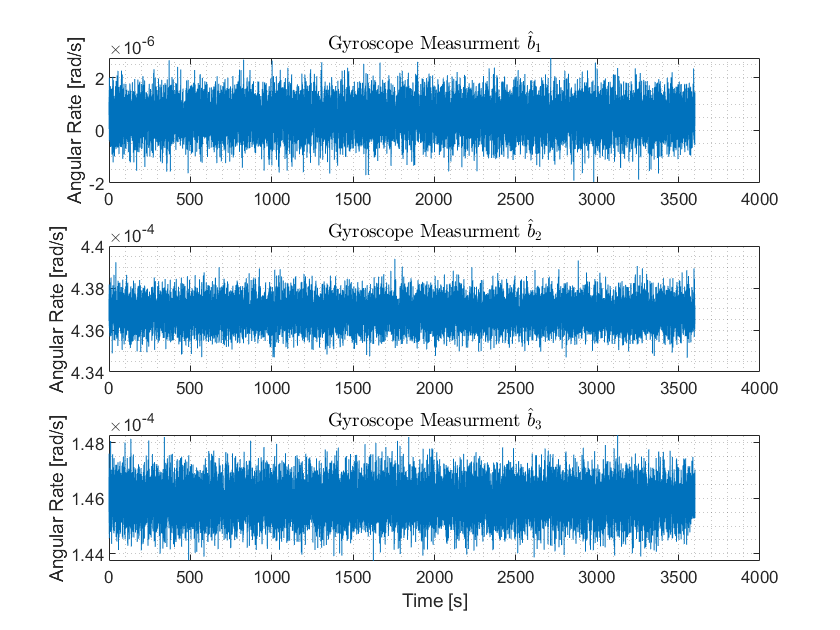
\includegraphics[height=5cm, keepaspectratio]{GyroOutput.png}
		\captionof{figure}{Gyroscope Measurments}
		\label{fig:ex1}
	\end{minipage}%
	\begin{minipage}{.5\textwidth}
		\centering
		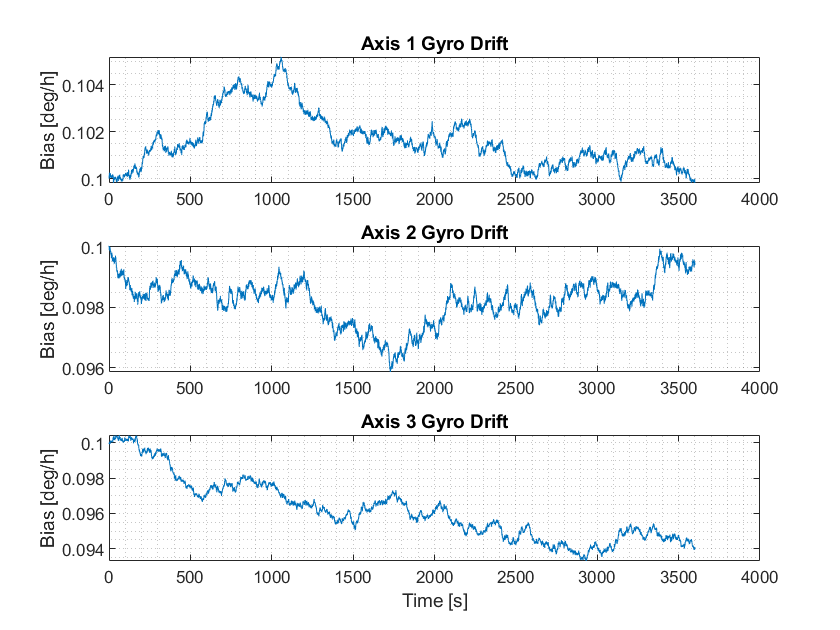
\includegraphics[height=5cm, keepaspectratio]{GyroBias.png}
		\captionof{figure}{Gyroscope Bias}
		\label{fig:ex2}
	\end{minipage}
\end{figure}

\noindent Similarly for the star tracker, using equation 7 and the parameters from tables 1 and 2, the star tracker measurements for each of the 5 stars was generated. A series of measurements for a single star is shown below, where it is plotted against the truth.  

\begin{figure}[h!]
	\centering
	\begin{minipage}{.5\textwidth}
		\centering
		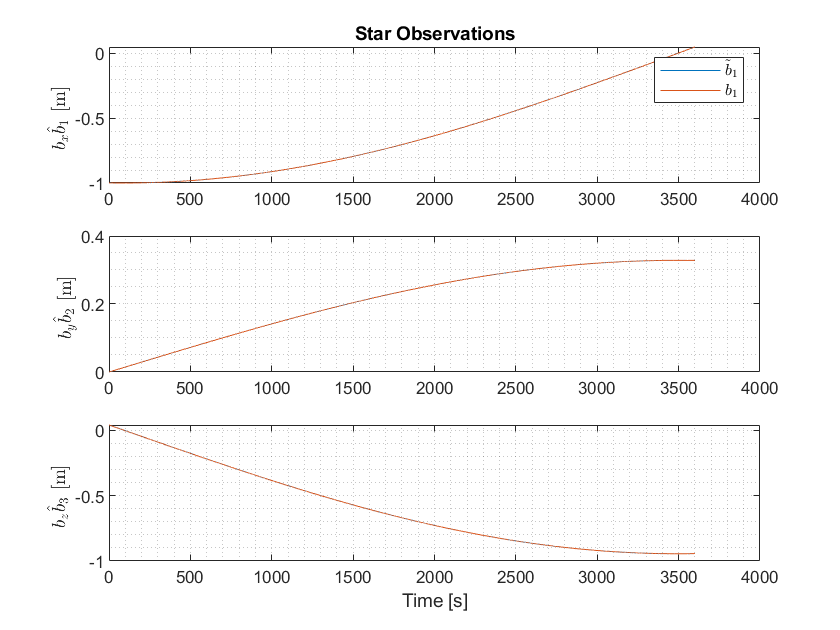
\includegraphics[height=5cm, keepaspectratio]{StarOutput.png}
		\captionof{figure}{Measurments for a Single Star}
		\label{fig:ex1}
	\end{minipage}%
	\begin{minipage}{.5\textwidth}
		\centering
		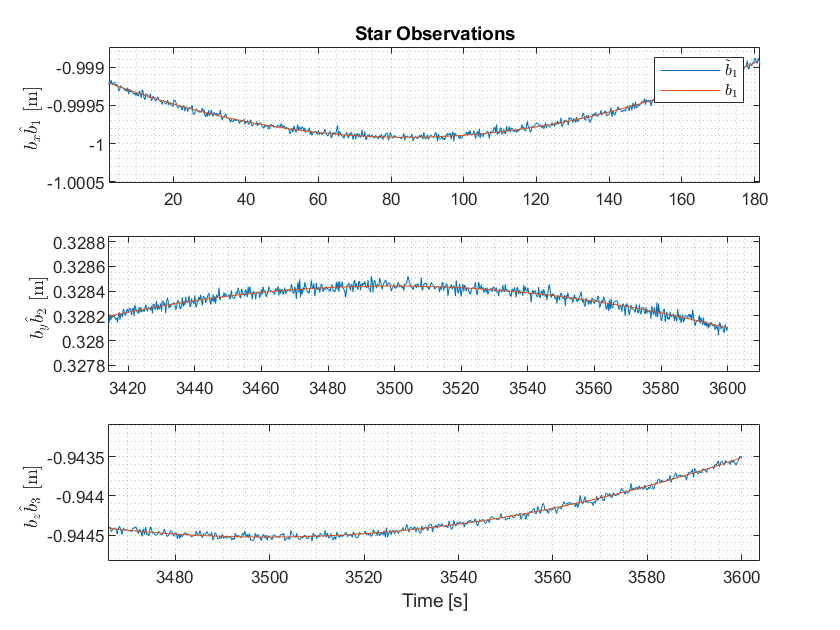
\includegraphics[height=5cm, keepaspectratio]{starnoise.png}
		\captionof{figure}{Zoomed In Measurment to Observe Noise}
		\label{fig:ex2}
	\end{minipage}
\end{figure}


\noindent As shown in table 1, all the sensors modeled are high quality sensors with small standard deviations. Due to this, it was necessary to zoom in on the measurements for the star tracker to see the noise as it was small compared to the change in trajectory. Both the gyroscope and star tracker were sampled at 4 Hz (slow for a gyroscope, fast for a star tracker). \\

\noindent Both the MEKF and the USQUE were initialized with the following state estimates and covariance: $\pmb{\hat{q}}_0 = \frac{\sqrt{2}}{2}[0, 1, 1, 0]^T$, $\hat{\pmb{\beta}}_0 = [0, 0, 0]^T$ [deg/hr], $P_0^a = 1$ [deg]$^2$, and $P_0^b = .05$ [deg/hr]$^2$. For the USQUE,the parameter \textit{a} was chosen to be 1, and $\lambda$ was tuned to be 5 as it gave the most accurate estimates of both the bias and the attitude. This value of \textit{a} with the previously mentioned expression for scale factor f, gives four times the vector of Modified Rodrigues Parameters used in the error parameterization [6]. Both the MEKF and USQUE are being given the same set of measurements, initial conditions and are also both updated at 4 Hz. It should be noted that there are non-zero initial condition errors for each state, so this run looks to compare the performance of both filters in response to the small initial condition errors provided to each filter. The estimates and errors for each filter is shown in the following figures.

\begin{figure}[h!]
	\centering
	\begin{minipage}{.5\textwidth}
		\centering
		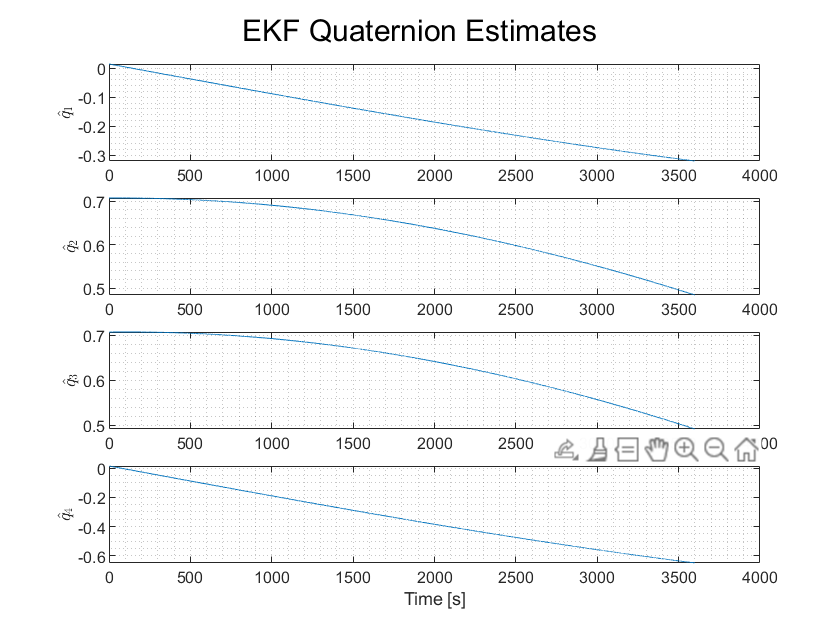
\includegraphics[height=5cm, keepaspectratio]{ekfQuatEst.png}
		\captionof{figure}{MEKF Quaternion Estimates}
		\label{fig:ex1}
	\end{minipage}%
	\begin{minipage}{.5\textwidth}
		\centering
		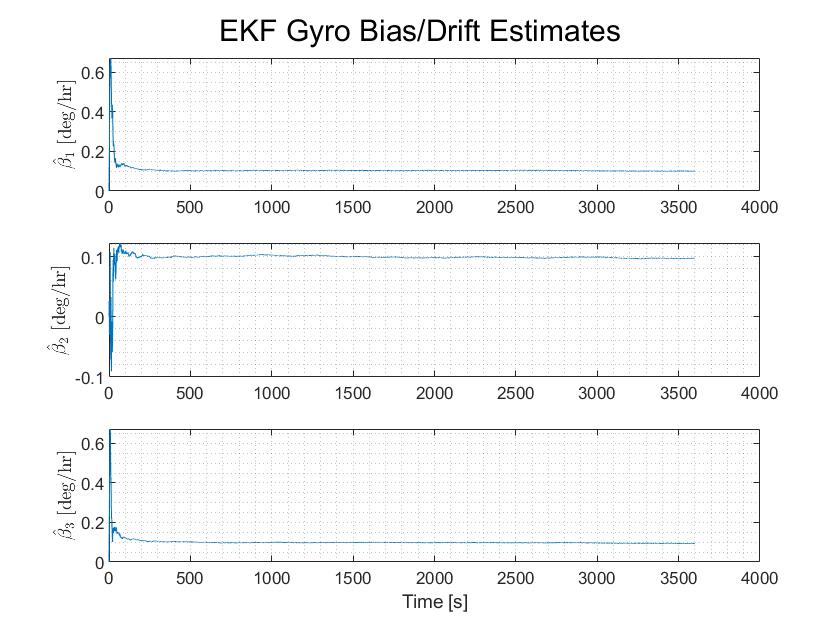
\includegraphics[height=5cm, keepaspectratio]{ekfBiasEst.png}
		\captionof{figure}{MEKF Bias Estimates}
		\label{fig:ex2}
	\end{minipage}
\end{figure}

\begin{figure}[h!]
	\centering
	\begin{minipage}{.5\textwidth}
		\centering
		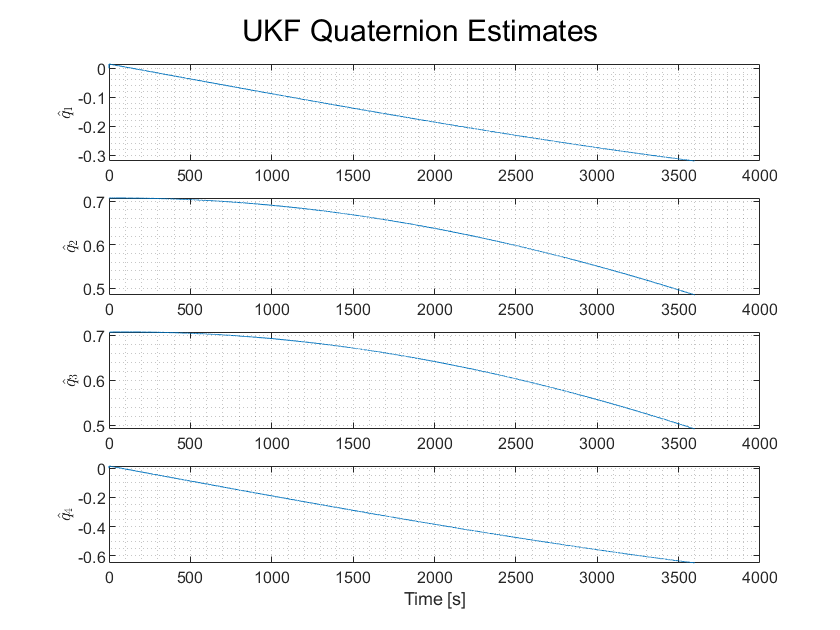
\includegraphics[height=5cm, keepaspectratio]{ukfQuatEst.png}
		\captionof{figure}{USQUE Quaternion Estimates}
		\label{fig:ex1}
	\end{minipage}%
	\begin{minipage}{.5\textwidth}
		\centering
		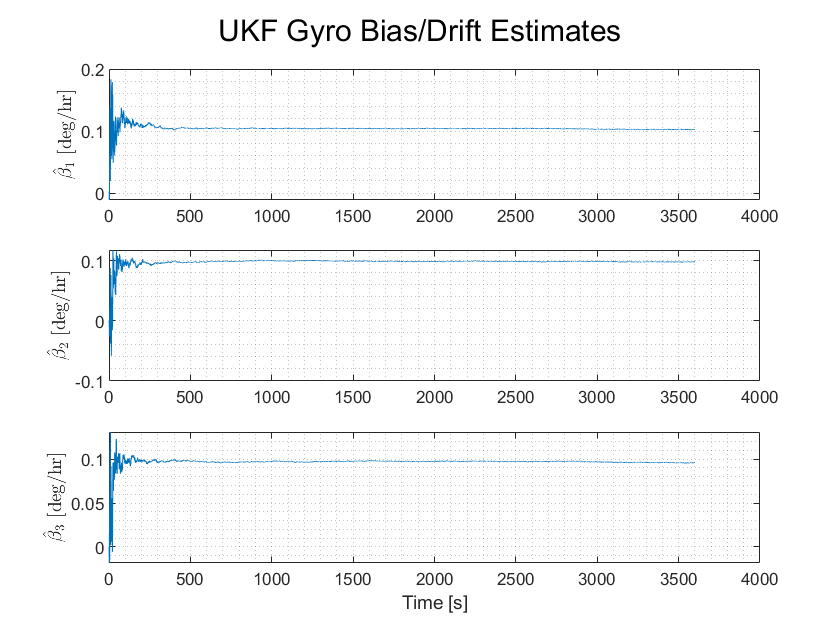
\includegraphics[height=5cm, keepaspectratio]{ukfBiasEst.png}
		\captionof{figure}{USQUE Bias Estimates}
		\label{fig:ex2}
	\end{minipage}
\end{figure}

\begin{figure}[h!]
	\centering
	\begin{minipage}{.5\textwidth}
		\centering
		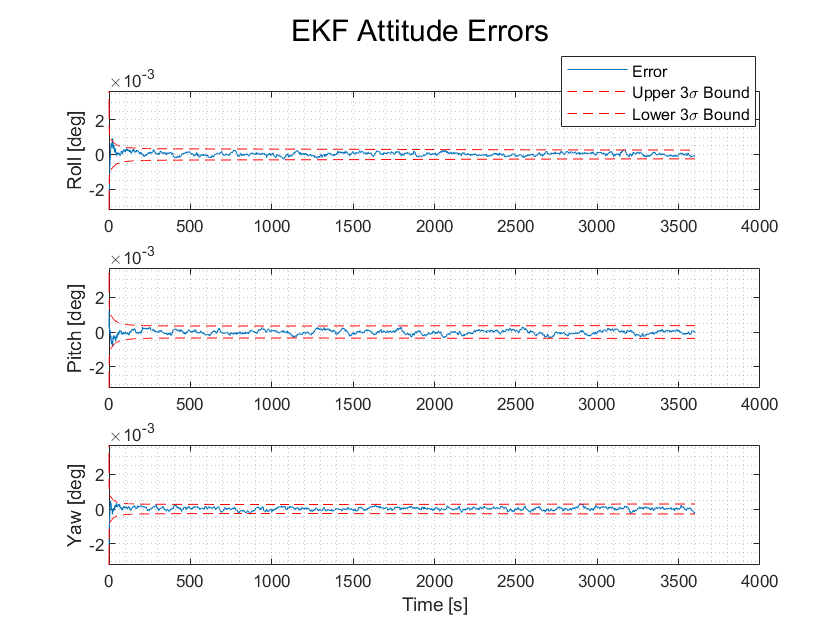
\includegraphics[height=5cm, keepaspectratio]{ekfAttErr.png}
		\captionof{figure}{MEKF Attitude Errors}
		\label{fig:ex1}
	\end{minipage}%
	\begin{minipage}{.5\textwidth}
		\centering
		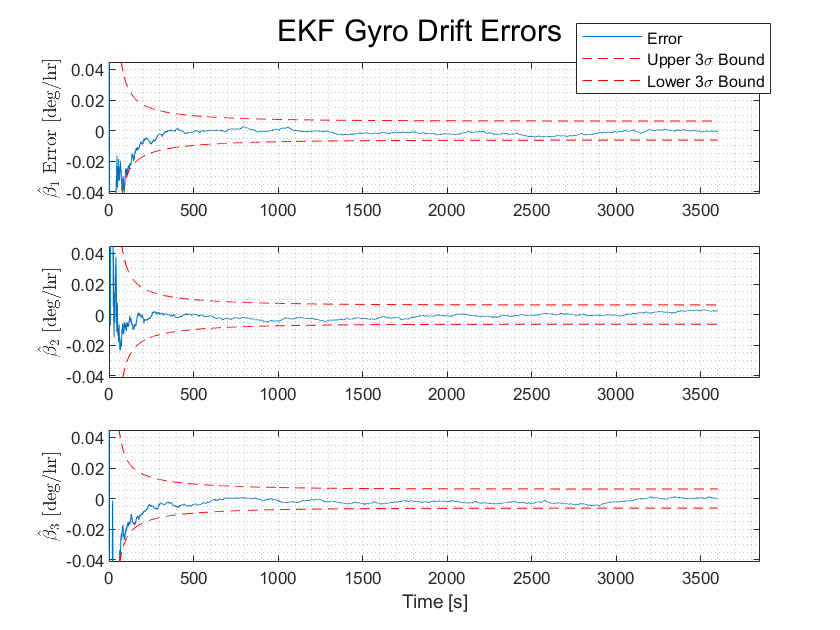
\includegraphics[height=5cm, keepaspectratio]{ekfBiasErr.png}
		\captionof{figure}{MEKF Bias Errors}
		\label{fig:ex2}
	\end{minipage}
\end{figure}

\begin{figure}[h!]
	\centering
	\begin{minipage}{.5\textwidth}
		\centering
		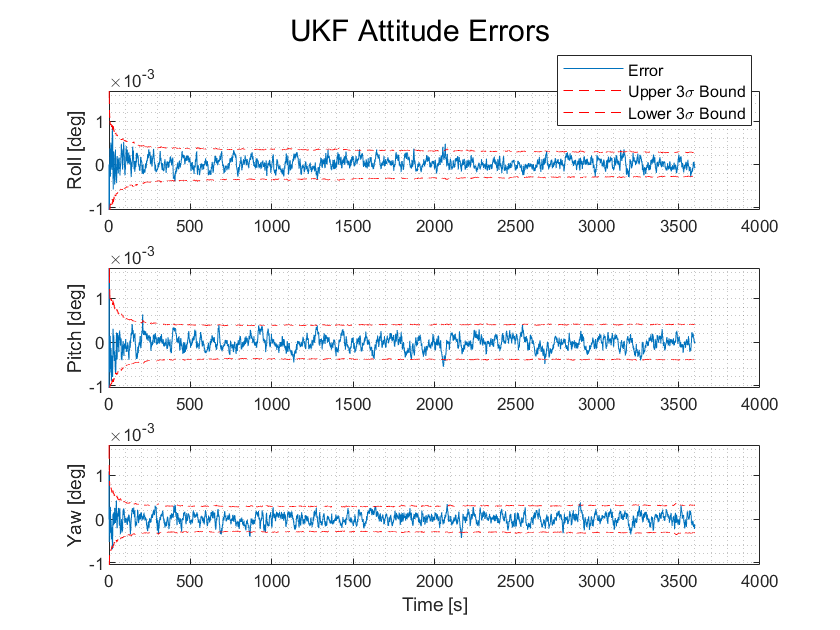
\includegraphics[height=5cm, keepaspectratio]{ukfAttErr.png}
		\captionof{figure}{USQUE Attitude Errors}
		\label{fig:ex1}
	\end{minipage}%
	\begin{minipage}{.5\textwidth}
		\centering
		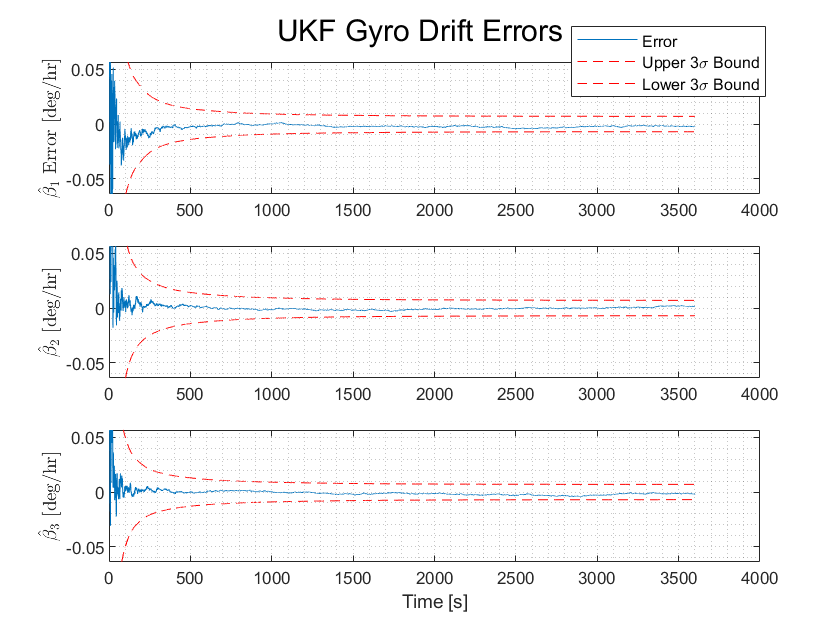
\includegraphics[height=5cm, keepaspectratio]{ukfBiasErr.png}
		\captionof{figure}{USQUE Bias Errors}
		\label{fig:ex2}
	\end{minipage}
\end{figure}
\newpage

\noindent From figures 10-13, it is observed that both the MEKF and USQUE attitude and bias errors converge quickly and are well bounded. The magnitudes of the attitude and bias estimates for both filters agree. The only major difference appears to occur in the beginning of the simulation, where the MEKF bias estimates jump to 0.6 deg/hr then converges, while the USQUE only reaches 0.2 deg/hr, as shown in figures 7 and 9. Zooming in on the initial filter performance shows the following.

\begin{figure}[h!]
	\centering
	\begin{minipage}{.5\textwidth}
		\centering
		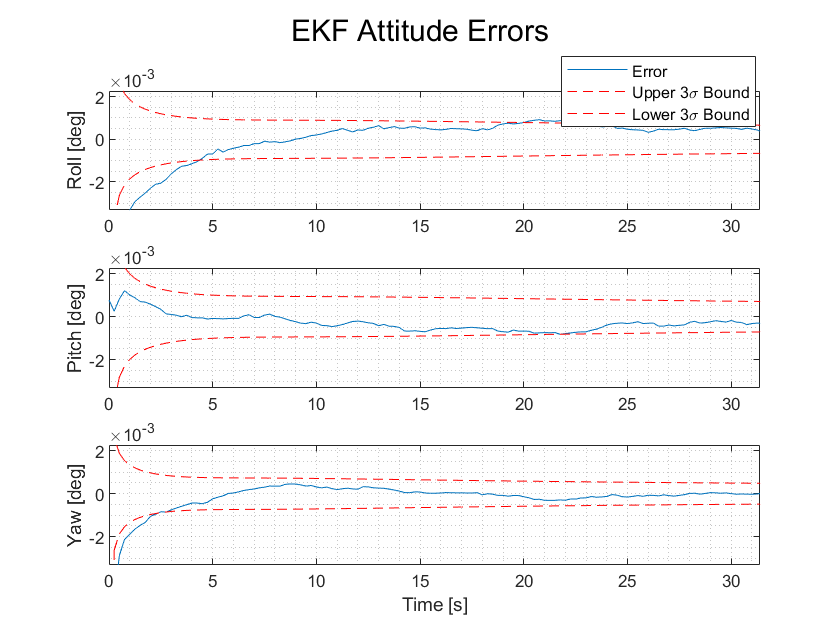
\includegraphics[height=5cm, keepaspectratio]{ekfAttErrBegin.png}
		\captionof{figure}{MEKF Attitude Errors - Beginning}
		\label{fig:ex1}
	\end{minipage}%
	\begin{minipage}{.5\textwidth}
		\centering
		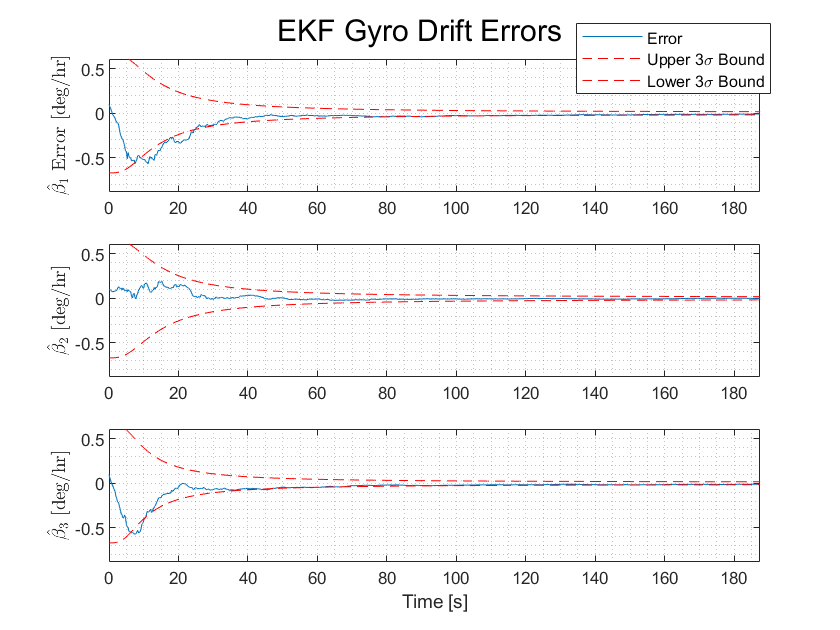
\includegraphics[height=5cm, keepaspectratio]{ekfBiasErrBegin.png}
		\captionof{figure}{MEKF Bias Errors - Beginning}
		\label{fig:ex2}
	\end{minipage}
\end{figure}

\begin{figure}[h!]
	\centering
	\begin{minipage}{.5\textwidth}
		\centering
		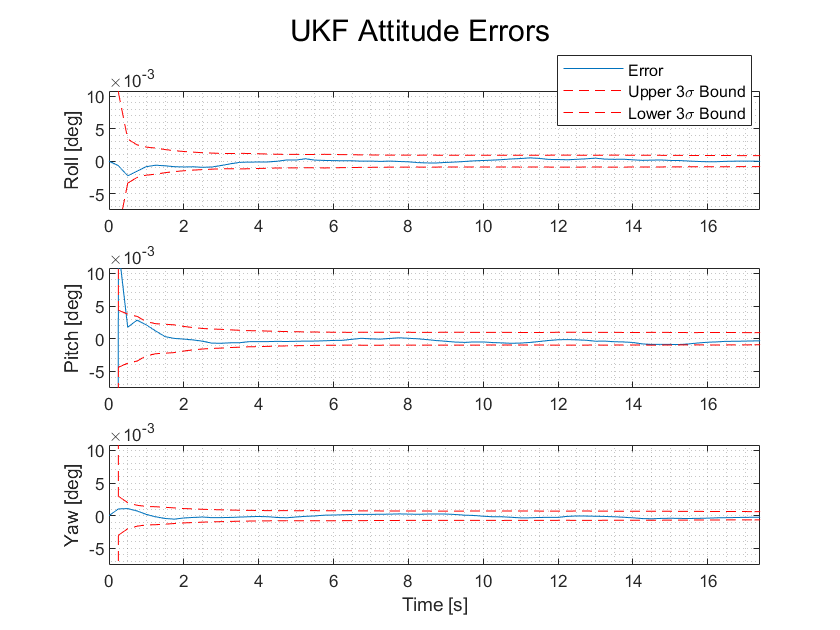
\includegraphics[height=5cm, keepaspectratio]{ukfAttErrBegin.png}
		\captionof{figure}{USQUE Attitude Errors - Beginning}
		\label{fig:ex1}
	\end{minipage}%
	\begin{minipage}{.5\textwidth}
		\centering
		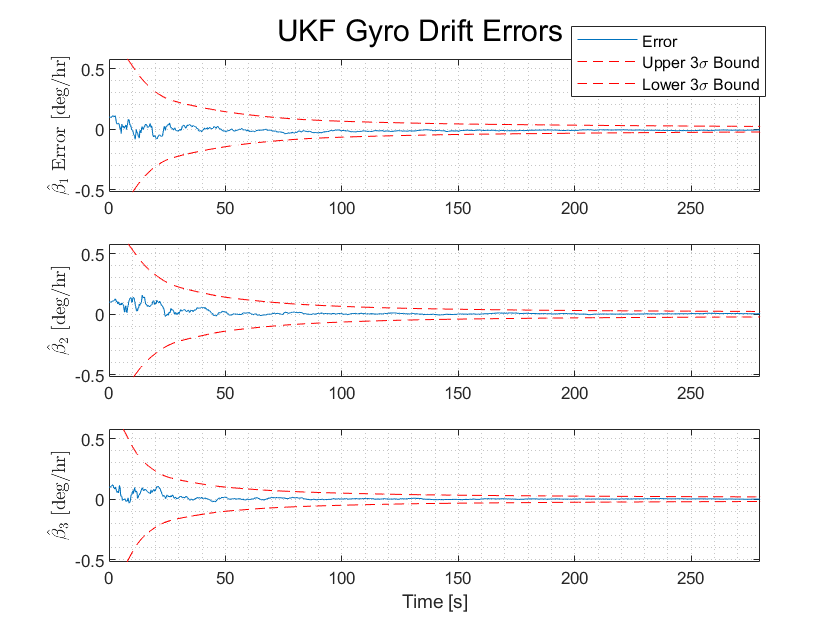
\includegraphics[height=5cm, keepaspectratio]{ukfBiasErrBegin.png}
		\captionof{figure}{USQUE Bias Errors - Beginning}
		\label{fig:ex2}
	\end{minipage}
\end{figure}

\noindent Figures 14 and 15 show that attitude errors for the MEKF take about 7 seconds for the errors to converge within the 3$\sigma$ error bounds. The MEKF bias errors on the other hand take approximately 40 seconds to converge within the 3$\sigma$ error bounds. Comparing this to the USQUE, it is observed in figures 16 and 17 that the attitude errors converge within the error bounds almost immediately, while the bias error is always well bounded. Due to this observation, it appears that USQUE does handle the initial condition errors better than the MEKF. Despite this, both filters do perform well as the state errors settle within their respective error bounds after the effects of the initial condition errors die off. Both filters provide similar and accurate estimates of the attitude quaternion and gyroscope bias, as both sets of the estimated quaternions line up with the true quaternion trajectory of figure 1, while both filters give an estimated gyro bias of around 0.1 deg/hr after 100 seconds. The figure below shows the mean state errors and the run time for each filter, where the USQUE takes almost 5 times as long to run as the MEKF. 

\begin{figure}[h!]
	\centering
	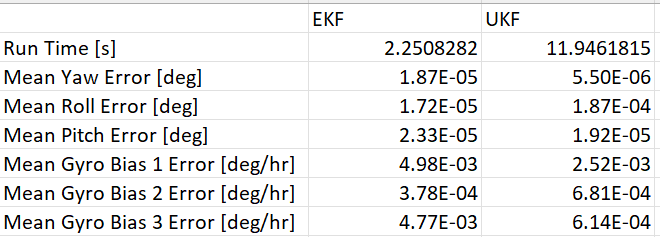
\includegraphics[width = .8\textwidth]{Table.png}
	\caption{Mean State Errors}
	\label{fig:Part B}
\end{figure}

\noindent From figure 18, the mean state errors appear to be comparable, with the only real differences being in the mean yaw and axis 3 gyroscope bias error where the USQUE outperforms the MEKF. However, this slightly improved error for a couple states may not be enough to warrant the significant difference in run time. A Monte Carlo simulation looks to investigate this further. Lastly, the quaternion error for both the MEKF and USQUE are shown below in figures 19 and 20, where it is observed that the scalar component of the quaternion, $q_4$, remains approximately constant with a value of 1. This matches with what is assumed from the first order approximation of equation 7.13 from ref [5], as previously mentioned. 

\begin{figure}[h!]
	\centering
	\begin{minipage}{.5\textwidth}
		\centering
		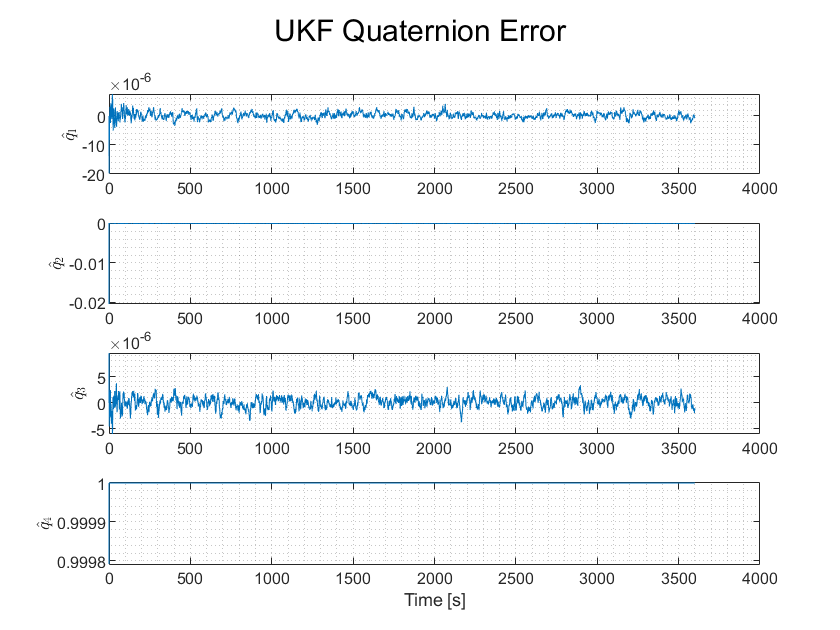
\includegraphics[height=5cm, keepaspectratio]{ukfQuatErr.png}
		\captionof{figure}{USQUE Quaternion Error}
		\label{fig:ex1}
	\end{minipage}%
	\begin{minipage}{.5\textwidth}
		\centering
		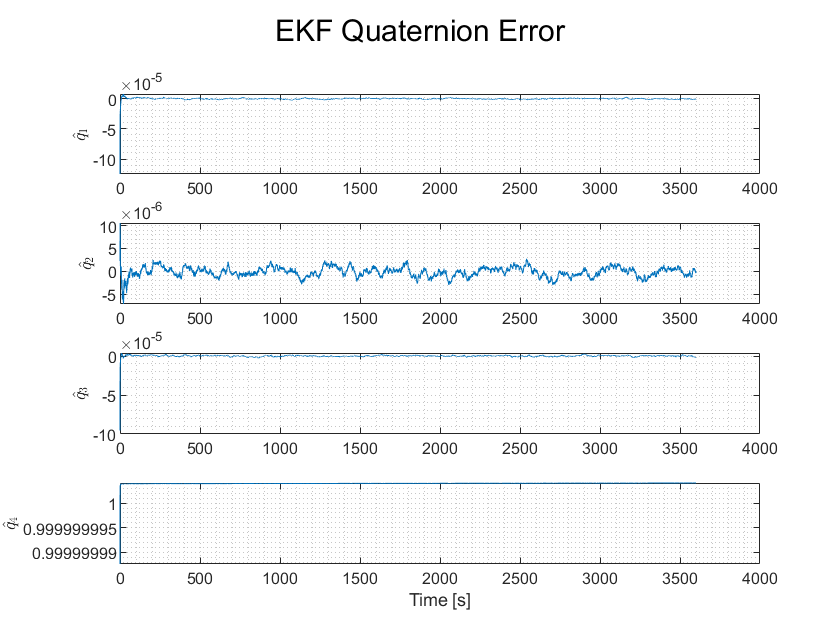
\includegraphics[height=5cm, keepaspectratio]{ekfQuatErr.png}
		\captionof{figure}{MEKF Quaternion Error}
		\label{fig:ex2}
	\end{minipage}
\end{figure}

\section*{Monte Carlo Run Simulation }
\addcontentsline{toc}{section}{Monte Carlo Run Simulation}
\noindent The initial bias and quaternion estimates were normally distributed with the mean given by $\pmb{\hat{q}}_0 = \frac{\sqrt{2}}{2}[0, 1, 1, 0]^T$ and $\hat{\pmb{\beta}}_0 = [0, 0, 0]^T$ [deg/hr]. Each component of both estimates were varied with a standard deviation of 0.05. The quaternion was normally distributed then re-normalized to maintain the unit norm. The initial attitude covariance was kept the same as before and the bias covariance was increased so $P_0^b = 0.2$ [deg/hr]$^2$. 100 Monte Carlo runs were performed and the sum of the norms of the attitude errors for each run were stored and compared between the MEKF and USQUE, where each run used the same set of measurements. The equation used to calculate this sum of the norm is given below, where $\alpha$ is a vector of error angles with yaw,pitch, and roll components. The results are given below. 

\begin{equation}
	y = \sum_{t = 0}^{3600}||\pmb{\alpha}(t)||
\end{equation}

\begin{figure}[h!]
	\centering
	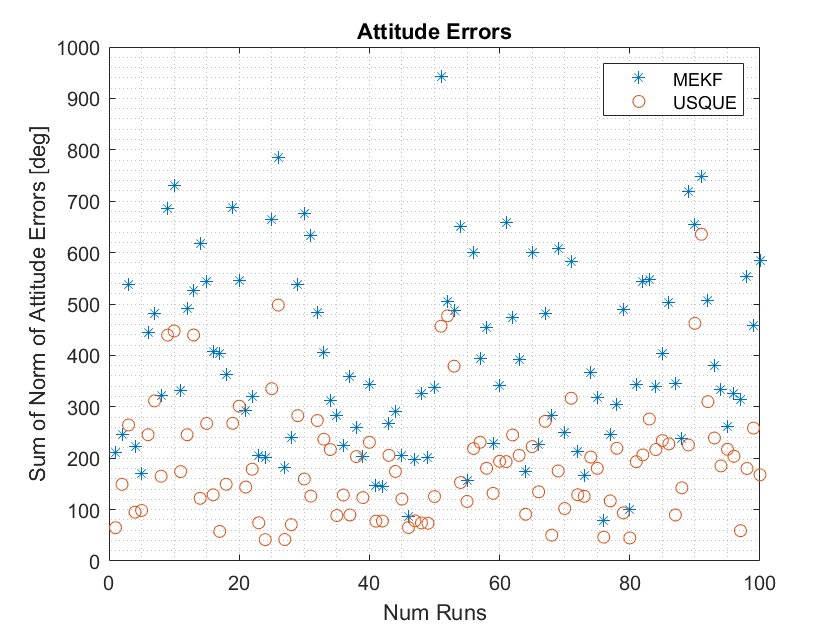
\includegraphics[width = .8\textwidth]{attErrMC.png}
	\caption{Mean State Errors}
	\label{fig:Part B}
\end{figure}

\noindent From figure 21, it is shown that for varying initial conditions, the USQUE repeatedly had lower attitude errors than the MEKF. The peak sum of the norm of the attitude error for the USQUE was around 650 deg, while the MEKF was around 950 deg. So this confirms that the USQUE does a better job of handling the initial condition errors than the MEKF. However, over the course of 100 runs, the mean run time for the MEKF was found to be 2.2 seconds, while the USQUE was found to have a mean run time of 12.4 seconds. This goes to show how much more computationally expensive the USQUE algorithm is in comparison to the MEKF. For a number of given initial estimates, the USQUE and MEKF had similar attitude error magnitudes of within 100 degrees of each other over the course of a 1 hour period. Taking the mean of all the summed norms of the attitude errors gives a mean norm of 397 degrees for the MEKF and a mean norm of 195 degrees for the USQUE. This shows the USQUE attitude errors have a lower magnitude by a factor of 2. However, these norms were summed over 3600 seconds, so this corresponds to the attitude errors having a norm of .05 degrees at each time step for the USQUE and .11 degrees for the MEKF. Obviously the USQUE still performs better by a factor of 2, but this difference in attitude error at each time step is not extremely large. Therefore, the MEKF may still be the more desirable with its much shorter run time.  

\section*{Conclusions }
\addcontentsline{toc}{section}{Conclusions}
\noindent In this paper, it was shown how to generate high fidelity pseudo-measurements for a star tracker and gyroscope. Using these measurements a quaternion parameterized Extended Kalman filter known as the MEKF and a quaternion parameterized Unscented Kalman filter known as the USQUE, were applied to an attitude estimation problem. Both filters used a multiplicative error quaternion that preserved the unit norm and used a reduced order state vector of length 6. This was done in the MEKF via the small angle approximation and a first order linearization, while the USQUE used generalized Rodrigues parameters to achieve the reduced order state. It was found that given initial estimates that had small initial condition errors, both filters gave good estimates with well bounded errors. It was also found that for both small and large initial condition errors, the USQUE marginally outperformed the MEKF as its attitude errors were smaller and converged quicker. The USQUE had a 5x longer run time than the MEKF, as it is more computationally involved. Both these findings lined up with what was expected from theory. The findings from this paper show that there is no definite end all filter to be used for attitude estimation problems, as it varies by situation. If the initial conditions are well known, than the MEKF will provide just as accurate estimates as the USQUE without the large computational load. If there is large initial uncertainty and the onboard computer can handle the computational load of an UKF, then the USQUE may be the filter for that scenario. 



\newpage
\section*{References}
\addcontentsline{toc}{section}{References}

\noindent [1] Schaub, H. and Junkins, J.L., \textit{Analytical Mechanics of Space Systems - Fourth Edition}, American Institute of Aeronautics and Astronautics, Reston, Virginia, 2018.\\
\noindent [2] Jekeli, C., \textit{Inertial Navigation with Geodetic Applications}, Walter de Gruyter, Berlin, Germany, 2000.\\
\noindent [3] Crassidis, J.L., “Sigma-Point Kalman Filtering for Integrated GPS and Inertial Navigation,” \textit{AIAA Guidance, Navigation and Control Conference and Exhibit},
San Francisco, California, August 2005.\\
\noindent [4] Markley, L. \textit{Multiplicative vs. Additive Filtering for Spacecraft Attitude Determination}, NASA Goddard Space Flight Center, Greenbelt, MD, 2004. \\
\noindent [5] Crassidis, J.L. and Junkins, J.L., \textit{Optimal Estimation of Dynamic Systems - Second Edition}, Chapman \& Hall/CRC, Boca Raton, FL, 2012.\\
\noindent [6] Crassidis, J.L. and Markley, F.L., "Unscented Filtering for Spacecraft Attitude Estimation," \textit{Journal of Guidance, Control, and Dynamics}, Vol. 26, No. 4, July-Aug. 2003, pp. 536-542.






\end{document}